\chapter{Související práce}\label{cha:souvisejici}

Pokusy o vytvoření automatické metody pro kompletní transkripci hudby se podle \cite{Poliner2007} objevují již od sedmdesátých let, z důvodu značné obtížnosti této úlohy, která strmě roste s každým dalším přidaným hlasem ve zkoumaném signálu, však dodnes jedná o otevřený problém. Z tohoto důvodu se od devadesátých let objevují práce, které se pokouší alespoň o částečný automatický popis některých muzikálních aspektů skladeb.

Jednou z prvních je práce týmu \cite{Goto1999}, který se záměrně omezuje na identifikaci jedné, nejhlasitější, spojité křivky fundamentní frekvence hlasu (F0) v omezeném frekvenčním rozsahu. Vzniklé transkripce pak sice nejsou kompletní, na druhou stranu je jejich získání výpočetně nenáročné a přitom poskytují sémanticky bohatý popis nahrávek, který je poměrně často shodný s melodií. Ustanovením úlohy pojmenované jako \uv{Predominant-F0 Estimation} (PreFEst), byly položeny základy pro vznik navazujících prací a soutěží zabývající se automatickým přepisem melodie.

Největší rozkvět v oboru začal od roku 2004. Uspořádáním první soutěže pro porovnání systémů pro automatický popis hudby v rámci konference ISMIR (ISMIR 2004 Audio Description Contest), se ustanovily priority, formalizovaly podmínky evaluace a byly sestaveny první kolekce dat pro testování algoritmů (\cite{Downie2010}). Soutěž se v následujícím roku přerodila do samostatné každoroční události, v níž soutěží stále více týmů v rostoucím počtu úloh. 

V této kapitole představíme existující metody a společné přístupy k řešení úlohy extrakce melodie. Nejprve úlohu dekomponujeme na podúlohy a pro tyto podúlohy uvedeme příklady přístupů existujících metod. V závěru kapitoly pak provádíme kvantitativní srovnání existujících metod na základě dat ze soutěže MIREX pro výběr replikovaných metod v této práci.

\section{Průzkum existujících metod}

Jen do soutěže MIREX se od roku 2005 přihlásilo 45 týmů s 62 různými metodami pro extrakci melodie, s různou mírou přesnosti přepisu. Mezi přístupy k tomuto problému tedy existuje veliká rozmanitost, jejíž kompletní popis přesahuje rámec této práce. Zaměříme se proto na společné rysy a celkové trendy v oboru. 

Shrnující práce od \cite{Poliner2007} a \cite{Salamon2014} se při charakterizaci systémů pro transkripci odkazují na příbuznou úlohu odhadu fundamentální frekvence monofonní nahrávky. Algoritmy pro monofonní tracking na základě vstupního signálu $x_{mono}(t)$ počítají \emph{funkci salience} $S_{x_{mono}}(f_\tau, \tau)$ pro každý krátký časový okamžik (okno) $\tau$ a frekvenci $f_\tau$. Výsledkem této funkce je relativní ohodnocení (příp. pravděpodobnost) jednotlivých frekvencí obsažených ve vstupním signálu, které značí, zda-li je daná frekvence fundamentální frekvencí znějícího hlasu. 

Pro zvýšení robustnosti vůči šumu, přeslechu, dozvuku a jiným vlivům, které zhoršují kvalitu odhadu salience, se využívá také spojitosti fundamentální frekvence. Pro zajištění kontinuity extrahovaných frekvenčních kontur se zohledňuje také faktor temporálních závislostí $C(\mathbf{f})$, jejímž vstupem je kandidátní kontura $\mathbf{f}$ a výstupem je ohodnocení této celé kontury na její spojitost. Například tato funkce může penalizovat odhady, ve kterých výstupní F0 často přeskakuje o oktávu, což je u skutečného signálu nepravděpodobné a naopak jde o častou chybu při výpočtu salienční funkce signálů se silnými sudými harmonickými frekvencemi.

Výstupem monofonního trackingu je posloupnost frekvencí s maximální saliencí a spojitostí, tedy posloupnost frekvencí, které jsou nejlépe ohodnocenými kandidáty na fundamentální frekvenci a zároveň tato celá sekvence má také vysoké ohodnocení spojitosti.

    $$\hat{\mathbf{f}} = \argmax_{\mathbf{f}}{[\sum_{\tau}{S_{x_{mono}}(f_\tau, \tau)} + C(\mathbf{f})]}$$

Přejdeme-li k úloze extrakce melodie, obecně se vstupní polyfonní signál $x(t) = x_m(t) + x_d(t)$ skládá ze směsi melodického hlasu $x_m(t)$ a hudebního doprovodu $x_d(t)$, cílem metod pro extrakci je z pohledu přepisu fundamentální frekvence zvýšení robustnosti algoritmu vůči mnohem výraznějšímu druhu šumu - hudebnímu doprovodu $x_d(t)$. Výstupem našeho systému tedy bude posloupnost odhadů frekvence v každém časovém okně vstupního signálu, reprezentovaná vektorem $\hat{\mathbf{f}}$:

    $$\hat{\mathbf{f}} = \argmax_{\mathbf{f}}{[\sum_{\tau}{S'_x(f_\tau, \tau)} + C'(\mathbf{f})]}$$

kde $f_\tau$ je frekvence na pozici $\tau$ ve vektoru $\mathbf{f}$. $S'_x(f_\tau, \tau)$ je upravená funkce salience, která při výpočtu zohledňuje vliv doprovodu a složka $C'(\mathbf{f})$ představuje ohodnocení celého průběhu melodie.

Spolu s odhadem frekvencí by také měl systém na výstupu určit úseky, ve kterých v nahrávce melodie zní a kdy nikoli. K výstupu tedy patří také vektor $\hat{\mathbf{v}}$, se stejným počtem složek jako $\hat{\mathbf{f}}$, který indikuje přítomnost melodie v každém časovém okně $\tau$.

Většina existujících metod sdílí podobnou základní strukturu při řešení extrakce, která se zakládá na popsané formalizaci. Prvním krokem je transformace zvuku do frekvenční domény a následný odhad znějících výšek tónů v polyfonním signálu (výpočet funkce salience), druhým krokem je pak zpracování těchto odhadů a výběr melodie (tedy zpřesnění výsledné $\hat{\mathbf{f}}$ pomocí $C'(\mathbf{f})$). Přístupy k řešení těchto dvou kroků již s konkrétními příklady nastíníme v dalších sekcích.

% \subsection{Odhad výšek tónů}

\subsection{Spektrální analýza}

Zvuk hraného tónu na melodickém nástroji je z fyzikálního pohledu periodická změna tlaku vzduchu. Perioda tohoto signálu se nazývá fundamentální frekvence (označujeme F0) a zpravidla je tento signál složen ze součtu řady sinusoid, jejichž frekvence jsou celočíselným násobkem fundamentální frekvence. V čase měnící se amplitudy těchto \emph{harmonických frekvencí} udávají hlasitost a barvu hlasu, výška první harmonické frekvence (tj. výška fundamentální frekvence) pak ve většině případů odpovídá posluchačem vnímané výšce tónu. 

\begin{figure}[h]\centering
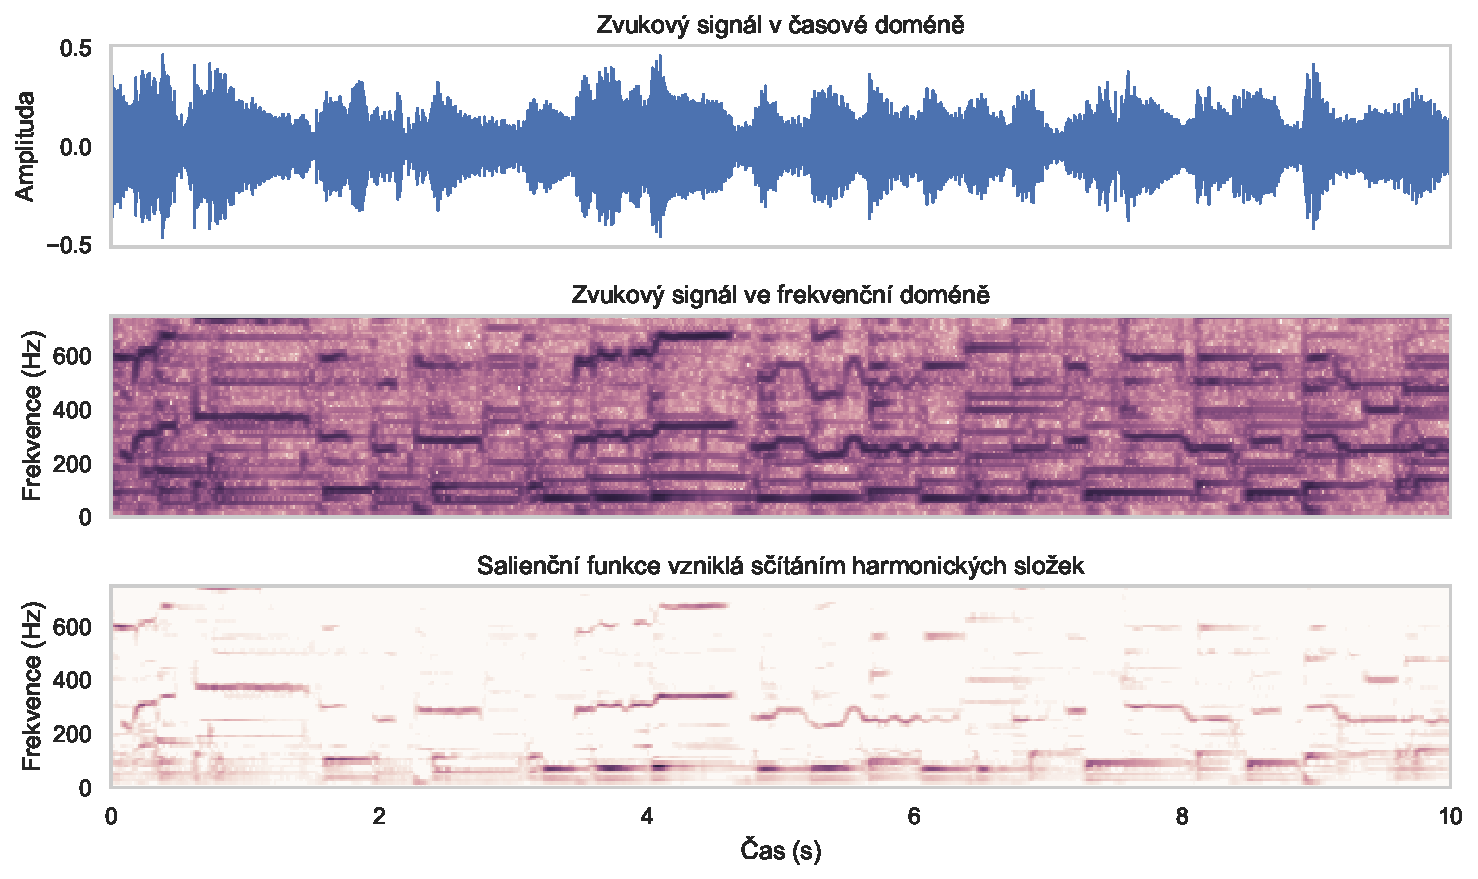
\includegraphics[width=\textwidth,height=\textheight,keepaspectratio]{../img/sig_spec_sal}
\caption{Znázornění kroků spektrální analýzy a výpočtu funkce salience.}
\label{obr:sig_spec_sal}
\end{figure}


Prvním krokem metod pracujících s hudebním signálem je proto provedení spektrální analýzy, jde o převod zvuku do frekvenční reprezentace, která odhaluje tyto harmonické struktury tónů a umožňuje s nimi dále pracovat. 

\subsubsection{Krátkodobá Fourierova transformace}

Přístupů ke spektrální analýze je více, přímočará a podle \cite{Dressler2016} nejčastěji používaná metoda je \emph{krátkodobá Fourierova transformace} (STFT). Jejím principem je rozdělení vstupního signálu na množinu překrývajících se oken konstantní délky a výpočet Fourierovy transformace těchto krátkých zvukových úseků. Komplexní výsledek transformace umocníme a získáme tzv. výkonové spektrum signálu, které obsahuje informaci o poměrech energie frekvencí, ze kterých se signál v okně skládá. Spektrogram $X(f, \tau)$ vypočteme v čase $\tau$ a frekvenční složce $f$ jako:

    % $$X(f, \tau) = \int_{-W/2}^{W/2}{w(t)y(\tau + t)e^{-j2\pi f t} \mathrm{d}t}$$

$$ X(f, \tau) = \abs{\sum^{\infty}_{n=-\infty}{x(n)w(n-\tau)e^{-2\pi i \cdot n \cdot f}}}^2 $$

Pro diskrétní vstupní signál $x(n)$ a okénkovou funkci $w(n)$. V této práci budeme pro výpočty spektrogramů používat Hannovo okno, které omezuje tzv. prosakování ve spektru. 

\[
w_{hann}(n) =
\begin{cases}
    \cos^2{\frac{\pi n}{N}}, & \text{pro} -\frac{N}{2} \leq n \leq \frac{N}{2},\\
    0, & \text{jinak}.
\end{cases}
\]

Kde $N$ je požadovaná velikost okna STFT tranformace (kvůli obvyklé praxi výpočtu STFT pomocí algoritmu rychlé Fourierovy transformace (FFT) se hodnota $N$ volí z $N \in \{512, 1024, 2048, \dots\}$).

\subsubsection{Logaritmická osa spektrogramu}

\begin{figure}[h]\centering
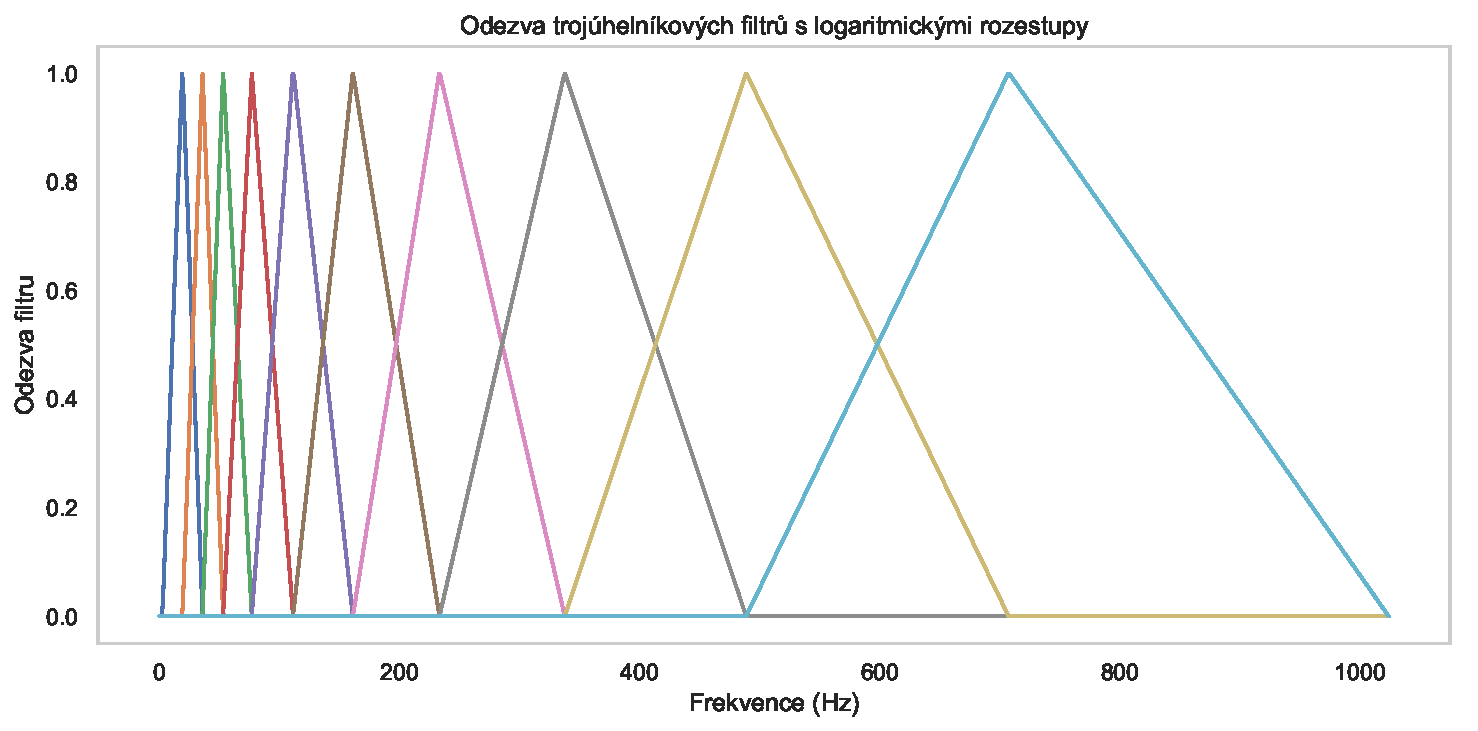
\includegraphics[width=\textwidth,height=\textheight,keepaspectratio]{../img/stft_triangular_filters}
\caption{Příklad trojúhelníkových filtrů pro transformaci frekvenční domény na logaritmickou škálu.}
\label{obr:stft_triangular_filters}
\end{figure}

Výsledkem STFT je rozložení signálu na jednoduché frekvenční složky (sinusoidy) s konstantně vzdálenými frekvencemi. Jinými slovy frekvenční osa spektrogramu vytvořeném metodou STFT je lineární. Jak jsme již nastínili v úvodu, povaha hudebních intervalů a harmonických struktur tónů spočívá v tom, že téměř všechny periodické signály se v hudební skladbě vyskytují ve vzájemných poměrech (v případě intervalů v poměrech $2^{\frac{n}{12}}$ a v případě harmonických frekvencí v celočíselných). K tónu, jehož základní frekvence je rovna $440\,\rm Hz$, patří také harmonické složky s frekvencemi $880\,\rm Hz$, $1320\,\rm Hz$, \dots, tedy absolutní vzdálenosti na spektrogramu STFT mezi frekvencemi harmonických složek jsou závislé na výšce základní frekvence. Toto způsobuje obtíže při analýze signálů, jelikož všechny uvažované frekvenční rozdíly jsou relativní. Častým druhem zpracování STFT je proto převod frekvenční osy na logaritmickou, na té pak platí pro vzdálenost libovolné fundamentální frekvence $f_0$ a její libovolné $h$-té harmonické frekvence $f_h = f_0 \cdot h$:

$$ \log{f_h} - \log{f_0} = \log{(h \cdot f_0)} - \log{f_0} = \log{h} + \log{f_0} - \log{f_0} = \log{h} = \rm const.$$

Tedy absolutní vzdálenosti uvnitř harmonické struktury tónů na spektrogramu s logaritmickou osou frekvence zůstávají konstantní nezávisle na výšce fundamentální frekvence. Tento přepočet se obvykle provádí pomocí banky filtrů s trojúhelníkovou odezvou, pro transformovaný signál $X(f, \tau)$ s $N$ frekvenčními složkami spočteme nový spektrogram s logaritmickou osou následovně:

$$ X_{\mathrm{log}}(\omega, \tau) = \sum^{\infty}_{f=-\infty}{g_\omega(f)X(f, \tau)}$$

Přičemž $g_\omega(f)$ značí odezvu trojúhelníkového filtru pro výstupní frekvenční složku $\omega$.

\subsubsection{Multirezoluční transformace}

Na libovolnou metodu převodu diskretizovaného signálu na frekvenční doménu se vztahuje Gaborův limit, který popisuje závislost přesnosti lokalizace signálu ve frekvenční a časové doméně \citep{Gabor1945}. Volbou délky vstupního okna transformace zpřesňujeme buď frekvenční nebo časové rozlišení výsledné spektrální reprezentace. Zvolíme-li krátké vstupní okno, zvyšujeme časové rozlišení (krátké okno lépe zachycuje rychlé změny průběhu signálu), avšak ztrácíme přesnost na frekvenční ose, opačný vztah platí pro volbu delšího okna.

Tato limitace je markatní zejména pokud STFT používáme pro hudební data. , u vyšších tónů jsou proto vzdálenosti mezi frekvencemi signálů větší než u nižších tónů. Frekvenční rozlišení STFT je však konstantní na celém výstupním frekvenčním rozsahu a volba velikosti okna transformace zajistí dobrý poměr frekvenčního a časového rozlišení jen pro část rozsahu. Ve výsledku je pak buď pro vyšší frekvence okno příliš velké (zbytečně detailní frekvenční rozlišení na úkor časového rozlišení) a nebo naopak pro nižší frekvence je okno nedostačující (rozlišení frekvence nemusí být pro basy ani na úrovni půltónů).

Z tohoto důvodu existují vedle STFT i další metody, jejichž cílem je nabídnout lepší kompromis frekvenčně-časového rozlišení v kontextu melodických dat. \cite{Goto1999} používají MRFFT (Multi-Resolution Fast Fourier Transform), principem je opakovaný downsampling signálu (převzorkování na nižší vzorkovací frekvenci) a aplikace Fourierovy transformace na každý vzniklý signál; s každou iterací spektrum obsahuje čím dál podrobnější informace o nižších frekvencích, protože vyšší frekvence se při downsamplingu ztratí. \cite{Brown1990} popsala metodu Constant-Q Transform (CQT), která spočívá v použití proměnné délky okna Fourierovy transformace pro výstupní frekvenční pásma, která rovnoměrně pokrývají logaritmickou osu frekvence. \cite{Cancela2010} kombinuje CQT a Chirp Z-transform, jedná se o zobecnění diskrétní Fourierovy transformace, ve které je signál rozložen na tzv. lineární čerpy --- sinusoidy s proměnnou frekvencí. Díky tomu transformace dokáže s lepším rozlišením zachytit signály, které rychle mění výšku tónu, v hudbě například vibrato. \cite{Paiva2004} napodobují mechanismy lidského sluchu pomocí banky pásmových filtrů (Cochleagram) s logaritmicky rozmístěnými mezními frekvencemi a sumy autokorelací na jednotlivých frekvenčních pásmech signálu (Summary correlogram).

I přes uvedené důvody se \cite{Salamon2014} a \cite{Dressler2016} domnívají, že metoda zpracování signálu příliš neovlivňuje výslednou přesnost algoritmů pro přepis melodie. Tvrzení dokládají jednak celkovým srovnáním výsledků metod ze všech ročníků soutěže MIREX a jednak neochvějnou převahou využití krátkodobé Fourierovy transformace, jakožto efektivní a dostačující metody pro spektrální analýzu.

\subsubsection{Postprocessing spektrogramu}

Po převodu signálu na frekvenční reprezentaci následuje u většiny metod některý druh úpravy celého spektrogramu, předcházející samotnému výpočtu \emph{funkce salience}. Výsledkem tohoto kroku může být potlačení šumu a nemelodických částí signálu, zpřesnění informace o výšce znějících frekvencí nebo normalizace či jiná úprava amplitud spektrogramu.

Nejčastější úpravou je nalezení lokálních maxim (vrcholů). Potlačením nemaximálních oblastí se zbavíme velkého množství nemelodických složek signálu, přitom informaci o těch melodických neztratíme. Výhodou práce s množinou vrcholů je, že jejich frekvenci lze na základě spektra dále zpřesnit pomocí parabolické interpolace (\cite{Rao2010}) a nebo využitím úhlové frekvence (\cite{Salamon2012a}, \cite{Dressler2009}). 

Jiným druhem úpravy jsou různé způsoby normalizace, ať jednoduché aplikace logaritmu na jednotlivé hodnoty spektrogramu (\cite{Cancela2008}, \cite{Bittner2017}) nebo složitější strategie normalizace, které se aplikují na celá výstupní okna krátkodobé Fourierovy transformace (spectral whitening, \cite{Ryynanen2008}), či které používají pohyblivé průměry nebo jinou metodu, beroucí v potaz širší zvukový kontext. Cílem normalizace je zvýraznění slabších harmonických frekvencí a potlačení celopásmových zvuků (například perkusí). Principiálně podobným krokem je aplikace pásmového filtru (\cite{Goto1999}) pro zvýraznění frekvencí obsahující melodii. Případně využití psychoakustických filtrů modelující lidské vnímání hlasitosti (\cite{Salamon2012a}, \cite{Ikemiya2016}). Ze signálu lze také oddělit melodické nástroje a perkusivní doprovod pomocí metod separace signálů (source separation). Používanými metodami jsou například Harmonic/Percussive Sound Separation (HPSS) (\cite{Tachibana2010}) nebo Robust principal component analysis (RPCA) (\cite{Ikemiya2016}).

\subsection{Funkce salience}

Salience tónu vyjadřuje míru důležitosti či nápadnosti ke svému hudebnímu okolí. Nejvíce ji ovlivňuje hlasitost v poměru ke zbylým znějícím hlasům, vliv má ale také řada dalších charakteristik hraní. \cite{Dressler2016} mezi příklady uvádí například frekvenční modulaci, jako je vibrato nebo glissando, zejména oproti frekvenčně stálému hudebnímu doprovodu (piano, kytara). Velký vliv má samozřejmě také i barva hlasu. Lidský zpěv nebo obecně zvuky se silnějšími vyššími alikvótními frekvencemi snadněji upoutají pozornost. V případě vícehlasu mají obecně posluchači potíže rozeznat výšky tónů uvnitř souzvuku. Pokud má posluchač přiřadit pociťovanou výšku tónu akordu, obvykle volí nejvyšší či nejnižší ze znějících frekvencí.

Výstupem funkce salience je ohodnocení každé výšky tónu v každém časovém okamžiku nahrávky, které co nejlépe odpovídá v relativních poměrech výše popsané zvukové salienci. Jelikož neexistují žádné studie, které by se zabývaly měřením a kvantifikací salience v hudbě, nelze posoudit, jak dobře výsledky obvyklých způsobů výpočtu funkce salience korelují s mírou, ze které vychází. \cite{Bittner2018a} se však domnívá, že odhad bude velmi hrubý, většina postupů totiž do výpočtu zahrnuje pouze hlasitost hlasu, a tedy vynechává řadu jiných důležitých faktorů, které salienci ovlivňují.

Přístupy k výpočtu by se daly zařadit do tří kategorií - sčítání harmonických frekvencí, odhad parametrů modelujících vstup a metody strojového učení. 

\subsubsection{Sčítání harmonických frekvencí}

Metody založené na sčítání harmonických frekvencí jsou principiálně nejjednodušší skupinou. Vychází z práce \cite{Hermes1988}, jejich podstatou je využití harmonické struktury zvuku tónů. Ohodnocení frekvence $f_\tau$ získáme váženou sumou amplitud všech jejích harmonických frekvencí $h \cdot f_\tau$. Pro spektrogram $X(f, \tau)$ signálu $x$, funkci vah $g(f_\tau, h)$ a $N_h$ počet zahrnutých harmonických frekvencí v sumě:

    $$S_x(f_\tau, \tau) = \sum_{h=1}^{N_h}{g(f_\tau, h)\abs{X(h \cdot f, \tau)}}$$

Pro ilustraci uvažme jednohlasý harmonický signál s fundamentální frekvencí $f^\star$. Hodnoty spektrogramu $X(f, \tau)$ tedy budou vyšší kolem frekvencí $H_{f^\star} = \{1\cdot f^\star, 2\cdot f^\star, 3\cdot f^\star, \dots\}$ a jinde nulové. Funkce $S_x(f, \tau)$ bude tedy pro $f \not\in H_{f^\star}$ nulová a v $f^\star$ bude nabývat globálního maxima. Příklad výstupu této metody pro polyfonní nahrávku je na obrázku \ref{obr:sig_spec_sal}.

\cite{Dressler2011} tuto metodu vylepšuje zpracováváním dvojic vrcholů vstupního spektrogramu, její výsledný salienční spektrogram obsahuje méně kandidátů na fundamentální frekvenci. \cite{Cancela2008} se pokouší zmenšovat chybné hodnoty salienční funkce pomocí vyhodnocení subharmonických frekvencí.

\subsubsection{Statistické modelování signálu}

\begin{figure}[h]\centering
    \includegraphics[scale=0.8]{../img/tone_model}
\caption{Ilustrace modelu tónu spolu se signálem, převzato z \cite{Marolt2004}}\label{obr:tone_model}
\end{figure}

Jiným přístupem k počítání funkce salience, který používá \cite{Goto1999}, je modelování okna spektrogramu váženým součtem harmonických struktur (modelů tónů). Snažíme se vrcholy ve spektru rozdělit mezi různě silně znějící tóny tak, aby v součtu co nejlépe odpovídaly měřeným intenzitám. Přístup se jinými slovy snaží zjistit, jaké tóny musely v danou chvíli znít, aby vzniklo dané spektrum. 

Vstupem metody je okno normalizovaného spektrogramu $p_X^{(t)}(x)$ v čase $t$. Okno se pokusíme modelovat jako hustotu pravděpodobnosti $p(x; \theta^{(t)})$ vzniklou váženou směsí modelů všech možných tónů melodie v definovaném rozsahu frekvencí v intervalu $[F_l, F_h]$. Hustotu pravděpodobnosti jednoho z tónů s fundamentální frekvencí $F$ označíme jako $p(x|F)$ (obrázek \ref{obr:tone_model} ukazuje jeden z možných modelů tónu), a jako $w^{(t)}(F)$ označíme váhu, kterou model tónu $p(x|F)$ přispívá do celkové smíšené hustoty pravděpodobnosti. Pak $p(x; \theta^{(t)})$ definujeme jako:

$$p(x; \theta^{(t)}) = \int_{F_l}^{F_h}{w^{(t)}(F)p(x|F) \mathrm{d}F}$$
$$\theta^{(t)} = \{\, w^{(t)}(F) \mid F_l < F < F_h \,\}$$

Cílem pak je nalezení takových parametrů $\theta^{(t)}$, aby model $p(x; \theta^{(t)})$ dobře popisoval pozorovaní $p_X^{(t)}(x)$. K tomu \cite{Goto1999} využívá Expectation-Maximization (EM) algoritmus. Výsledné parametry $\theta^{(t)}$ jsou pak hodnoty salienční funkce.

% \textcolor{red}{TODO: popsat Durrieu, jakožto jiný přístup k modelování signálu}

\subsubsection{Metody strojového učení}

K výpočtu funkce salience můžeme využít také metody strojového učení. První práci využívající těchto metod představují \cite{Poliner}, kteří úlohu formulují jako klasifikační. Vstupní okno signálu jejich metoda klasifikuje do jednotlivých tříd tónů melodie, výstup je tedy kvantizován na rozlišení jednoho půltónu. Pro tento účel využívají metodu podpůrných vektorů (SVM) přičemž vstupními příznaky je část spektrogramu signálu, konkrétně vektor s 256 složkami, který získávají pomocí krátkodobé Fourierovy transformace podvzorkovaného signálu. Metoda dosahovala průměrných výsledků v soutěžích MIREX 2005 a 2006. Strojové učení se v oboru příliš neuchytilo, z důvodu nedostupnosti dat, ale možná také i kvůli limitacím, které \cite{Poliner} ve své práci prezentují.

V roce 2016 na tyto nedostatky odpovídá práce \cite{Kum2016}. Augmentací dat a zaměřením se na odhad výšky zpěvu místo melodie úspěšně překovávají problém nedostatku dat. Místo klasifikátoru SVM používají hluboké neuronové sítě (3 skryté plně propojené vrstvy) a problém kvantizace na úroveň půltónu řeší natrénováním tří nezávislých sítí s různě jemným rozlišením výstupu, které pak spojí v jeden výstup. V jejich případě platí, že jemná síť má sice lepší výstupní rozlišení, celkově má ale horší přesnost, naopak je tomu u sítě s hrubým rozlišením, proto jejich výsledky kombinují a dosahují tehdejších state-of-the-art výsledků na vokálních datech. Podobný postup v tomtéž roce podniká i tým \cite{Rigaud2016}, podobně jako v práci \cite{Kum2016} se tým omezuje na odhad výšky zpěvu, používá augmentaci dat, přechází na hlubokou neuronovu síť (2 skryté plně propojené vrstvy) a používá jemnější rozlišení výsledného vektoru pravděpodobnostního rozdělení znějící výšky. Rozdílem je ale předzpracování dat pomocí dekompozice na harmonické a perkusivní složky pomocí HPSS. Práce \cite{Balke2017} používá neuronovou síť s jednou skrytou vrstvou pro anotaci jazzových sól ze spektrogramu s logaritmickou osou frekvence. 

\cite{Bittner2017} představuje první pokus o použití hlubokých sítí na úlohu extrakce melodie bez zaměření na zpěv. Úlohu formuluje jako odstranění šumu obrázku, cílem je ze vstupního spektrogramu pomocí hluboké sítě s konvolučními vrstvami vytvořit salienční funkci. Vstupní a výstupní data mají tedy stejné měřítko, výstup však v ideálním případě obsahuje pouze informace o fundamentálních frekvencích znějící melodie. Velmi přínosný je také popis vstupní spektrální reprezentace HCQT, která spočívá ve výpočtu několika CQT spektrogramů (kanálů), jejichž počáteční frekvence jsou vzdálené v harmonických poměrech, tudíž (protože CQT spektrogram používá logaritmickou osu frekvence) všechny související harmonické složky na celém spektru jsou na těchto spektrogramech zarovnané nad sebou v ose kanálů. Tento koncept je hlouběji popsán v kapitole Experimenty v sekci HCNN, kde tento nápad aplikujeme nejen na vstupní spektrogram, ale nově také na propojení celé neuronové sítě. Dalším důležitým přínosem práce je úprava reprezentace cílové salienční funkce pomocí rozostření hranic cílové výšky tónu. Zatímco předchozí metody trénovali sítě jako diskrétní klasifikaci s jednou správnou výstupní třídou, v této práci je cíl trénování gaussián se střední hodnotou uprostřed výšky tónu.

Práce \cite{Bittner2017} dokázala překonat state-of-the-art metody pouhým výpočtem salienční funkce. Metoda tedy úplně přeskakuje vyhlazování odhadů v čase a používá pouze nejzákladnější metody pro detekci melodie pomocí práhování. Zároveň však její salienční funkce pro odhad jednoho okna délky $\approx 11\,\rm ms$ zpracovává přibližně $150\,\rm ms$ vstupního okna, tedy v porovnání s existujícími metodami její salienční funkce zpracovává velmi široký kontext, proto není vyhlazování jejich výsledků nezbytné.

\cite{DBasaranSEssid2018} na této práci buduje a jednak prozkoumává možnosti použití jiné vstupní spektrální reprezentace (založené na práci \cite{Durrieu2011a}) a jednak do architektury sítě zabudovává rekurentní neuronové sítě, které zajišťují zmiňované vyhlazování odhadů. Jeho metoda překonává výsledky \cite{Bittner2017}, nevýhodou jeho přístupu je však hrubý výstup s rozlišením na půltóny.

V rámci soutěže MIREX také přibývají od roku 2016 nové metody založené na hlubokých sítích, ty se však buď stále zaměřují pouze na extrakci zpěvu (například \cite{Su2018}) případně k nim nelze dohledat související článek (v roce 2016 metody účastníka Zhe-Cheng Fan a v roce 2018 metoda od týmu Sanguen Kum, Juhan Nam).

\subsection{Hledání melodie}

Po výpočtu funkce salience $S_x(f_\tau, \tau)$ máme k dispozici odhady fundamentálních frekvencí v signálu, z těchto ohodnocení pak musíme vybrat výslednou konturu melodie. V závislosti na způsobu výpočtu funkce salience tyto ohodnocení frekvencí více či méně odpovídají jejich důležitosti v signálu. Triviálním řešením zpracování těchto hodnot by bylo vybrat frekvence s maximální saliencí pro každé časové okno $\hat{f}_\tau = \argmax_{f_\tau}{S_x(f_\tau, \tau)}$, tento jednoduchý přístup však nevolí mnoho metod, protože jeho výstup má u složitějších skladeb tendenci \uv{přeskakovat} mezi doprovodem a melodií.

Obecně se dají přístupy rozdělit na pravidlové metody a statistické metody, dále se pak metody liší v tom, zda na základě salienční funkce vytváří abstraktnější popisy obsahu - ať už na úrovni jednotlivých celistvých konturů, tónů nebo celých frází.

\cite{Goto1999} pro sledování melodie používá množinu \uv{agentů}, pohybujících se v čase po výstupu salienční funkce a na základě předem definovaných pravidel jejich pohyb zaručuje kontinuitu výstupní fundamentální frekvence. Podobné sledování kontur v čase na základě salienční funkce využívá i \cite{Dressler2009}. Jinou pravidlovou metodou je opakované nalezení globálního maxima, jeho iterativní prodlužování v obou směrech časové osy a následné vymazání této nalezené kontury z výstupu salienční funkce, čímž dovolíme nalezení nového globálního maxima (\cite{Cancela2008}, \cite{Salamon2012a}). Z extrahovaných kontur následně můžeme vybrat ty, které splňují kritéria pro melodické kontury.

Jiným přístupem k hledání melodie je použití statistických metod, jako je například modelování pomocí skrytých Markovových modelů. Na salienční funkci tyto metody pohlíží jako na sérii pozorování a pomocí hledání nejpravděpodobnější cesty skrz stavy modelu s vhodně nastavenými či z dat získanými pravděpodobnostmi přechodu získávají vyhlazenou konturu melodie. Tyto modely mohou být velmi komplexní a můžou zahrnovat modely průběhu not \citep{Ryynanen2008} nebo naopak velmi minimalistické, zahrnující pouze stavy pro jednotlivé tóny (\cite{Yeh2012})

\subsubsection{Přítomnost melodie (voicing)}

Důležitou součástí algoritmů pro extrakci melodie je detekce melodie v signálu. Většina metod tento krok provádí na konci vyhodnocování pomocí pevně nastaveného či dynamického práhování, jiné metody detekci melodie řeší filtrováním melodických kontur (\cite{Salamon2012a}). V případě statistických metod je stav neznějící melodie často přímo zabudován do statistického modelu \citep{Ryynanen2008}. Některé metody také používají klasifikační metody strojového učení \citep{Rigaud2016}.

\section{Srovnání existujících metod}

Pro celkové kvantitativní srovnání metod jsme zpracovali výsledky všech ročníků soutěže MIREX. Tuto soutěž a používané datasety blíže popisujeme v kapitole \hyperref[chap:evaluace]{Metody evaluace}. V této sekci prezentujeme shrnutí výsledků metod, pro které existují výsledky na všech evaluačních datasetech soutěže MIREX, vybíráme tedy převážně z metod od roku 2015, kdy byl vydán doposud nejnovější evaluační dataset ORCHSET. Díky práci \cite{Bosch2014}, který starší metody spustil na svém datasetu ORCHSET, můžeme ke srovnání přidat také výsledky metod \cite{Dressler2009}, \cite{Salamon2012a} a \cite{Durrieu2010}. Celkové srovnání nalezneme v tabulce \ref{obr:mirex_results}. Na základě těchto výsledků vybíráme metodu \cite{Salamon2012a} jakožto zástupce metod, které nejsou založeny na strojovém učení\footnote{metoda \cite{Dressler2009} nemá zveřejněnou implementaci.}.

\begin{figure}[h]\centering
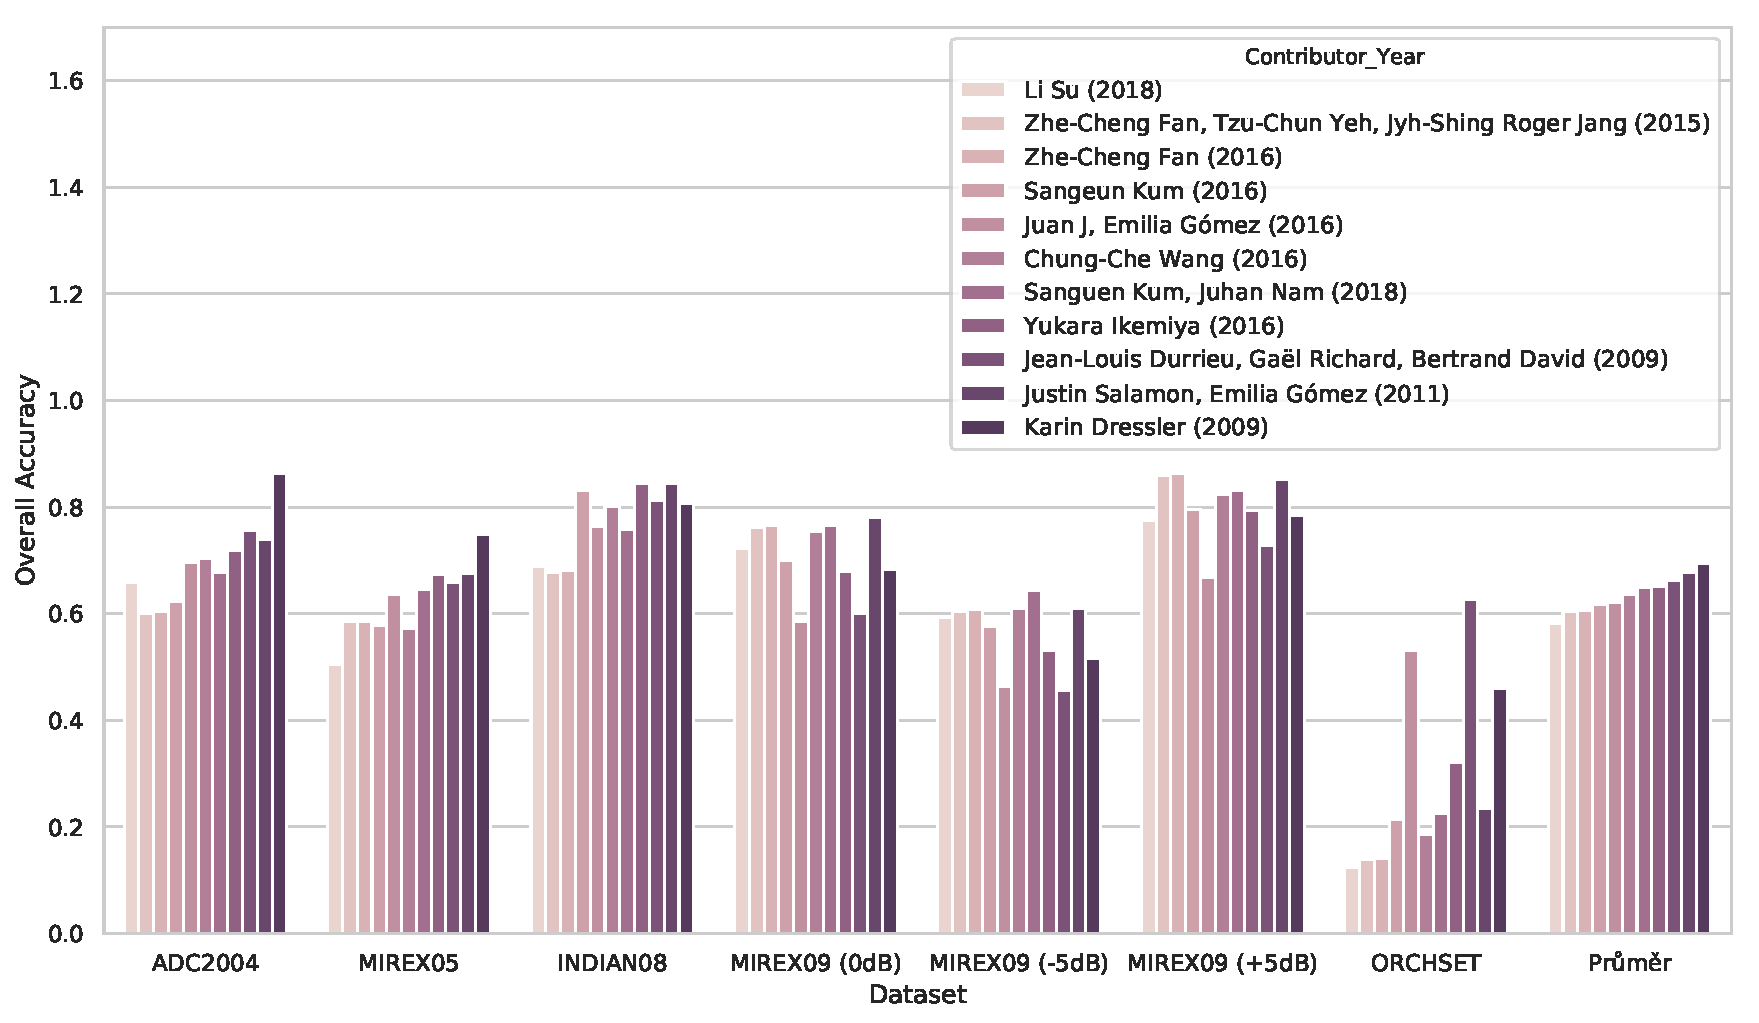
\includegraphics[width=\textwidth,height=\textheight,keepaspectratio]{../img/mirex_results}
\caption{Výsledky metod v soutěži MIREX v letech 2015-2018 s vybranými metodami ze starších ročníků.}
\label{obr:mirex_results}
\end{figure}

Na základě grafu \ref{obr:mirex_results} také vidíme, že největší variabilitu mají výsledky na datasetu ORCHSET, zde mají metody velký prostor pro zlepšení, naopak u datasetů INDIAN08 a variant MIREX09 je zřejmá jistá hranice kterou je pro metody obtížné překonat. \cite{Salamon2014} ve svém přehledovém článku dochází k závěru, že vývoj metod extrakce melodie začal od roku 2009 stagnovat, na obrázku \ref{obr:mirex_results_cumulative} znázorňujeme maximální dosaženou celkovou přesnost metod na jednotlivých datasetech od počátku soutěže MIREX. Bohužel musíme konstatovat, že v rámci soutěže MIREX stagnace pokračuje doposud, přitom výzkum metod stále pokračuje a zejména díky strojovému učení se obor posouvá. V rámci MIREXu však nebyly vyhodnoceny nové stěžejní metody \cite{Bittner2017} a \cite{DBasaranSEssid2018} a zájem o soutěž v této kategorii postupně upadá (v roce 2017 nesoutěžily žádné týmy, v roce 2018 pouze dva). Důvodem může být právě nedostatečný prostor pro zlepšení kvůli nedostatku nových, zajímavých dat.

\begin{figure}[h]\centering
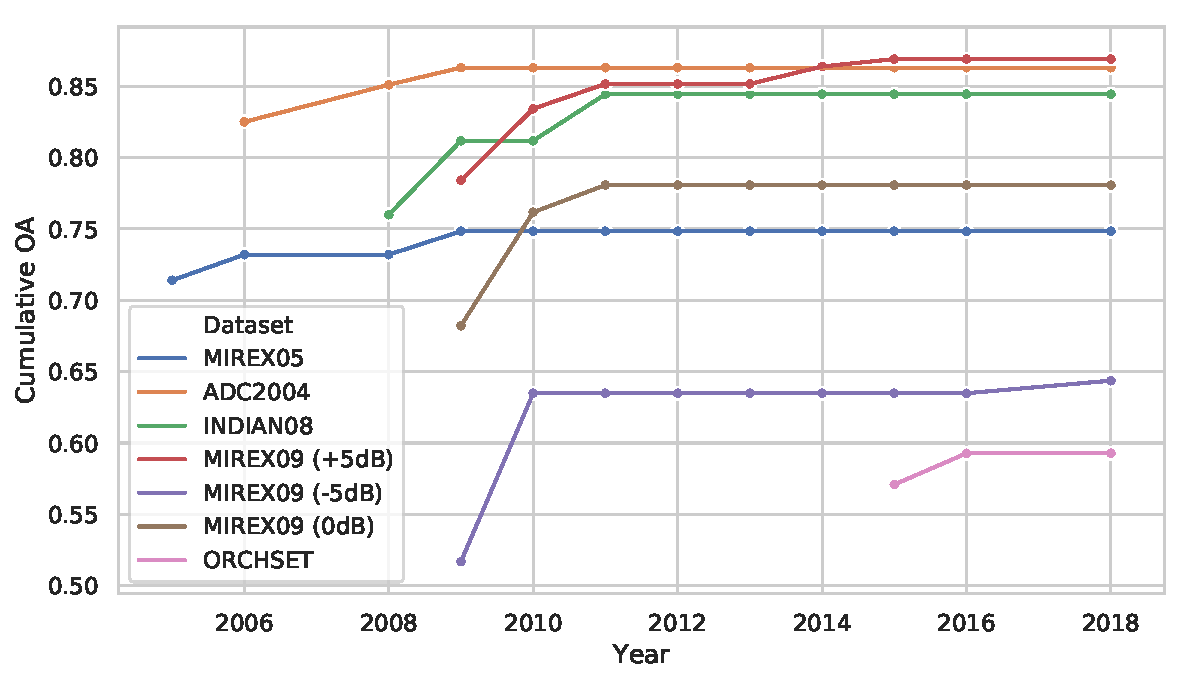
\includegraphics[scale=0.5]{../img/mirex_results_cumulative}
\caption{Stagnující vývoj metod pro extrakci melodie.}
\label{obr:mirex_results_cumulative}
\end{figure}

\subsection{Replikace výsledků}

Pro srovnání metod představovaných v této práci spouštíme metody \cite{Salamon2012a}, \cite{Bittner2017} a \cite{DBasaranSEssid2018} na testovacích množinách. Všechny tři metody mají volně dostupnou implementaci, první ve formě VAMP plug-inu\footnote{\url{https://www.upf.edu/web/mtg/melodia}}, zbylé jsou implementovány v jazyce Python a používají standardní knihovny určené pro hluboké učení\footnote{\url{https://github.com/rabitt/ismir2017-deepsalience/}}\footnote{\url{https://github.com/dogacbasaran/ismir2018_dominant_melody_estimation}}. Výsledky těchto metod uvádíme v kapitole Výsledky.

Poznamenáme, že implementace algoritmu \cite{Salamon2012a} existují dvě, druhá v rámci knihovny Essentia\footnote{https://essentia.upf.edu/documentation/}, tato implementace však v porovnání s implementací VAMP podávala výrazně horší výsledky napříč datasety. V kapitole Výsledky proto používáme implementaci VAMP.

Pokusili jsme se také o replikaci výsledků \cite{Bosch2014}, bohužel se nám ale kvůli nekompatibilitě mezi verzemi knihoven nepodařilo tuto 5 let starou metodu spustit. Teprve nedávno tuto chybu autoři odstranili\footnote{\url{https://github.com/juanjobosch/SourceFilterContoursMelody/commit/6f88e709c470f1423dc429198cb3c261a772c66c}}, výsledky již ale do práce nezahrnujeme z časových důvodů.

Pro srovnání jsme se také pokusili spustit metodu \cite{Durrieu2010}, délka běhu algoritmu je však při zachování výchozího nastavení parametrů neúnosně dlouhá, 23 minut dat (ORCHSET) nám trvalo zpracovat dva dny. Tudíž její spuštění na větší korpusy (MedleyDB, WJazzD) je mimo možnosti autora práce.

% \textcolor{red}{TODO: tabulka metod s popisem architektury}